\documentclass[12pt,compress,ngerman,utf8,t]{beamer}
\usepackage{etex}
\usepackage[ngerman]{babel}
\usepackage{graphicx}
\usepackage[export]{adjustbox}
\usepackage{multicol}
% \usepackage{animate}
% \usepackage{media9}


\usetheme[numbering=fraction, progressbar=frametitle]{metropolis}


\date{\today}
\institute{University of Freiburg}
\titlegraphic{\vspace{4cm} \hspace{9cm} 
\includegraphics[height=2cm]{template/Logo-Uni-Freiburg.png}}
\graphicspath{ {./template/} {./zsm/} }

\title{Selbstmanagement-Kompetenz}
\author{Janika, Maike, Charlotte, Felix}

\newif\ifonline
\onlinefalse
% \onlinefalse

\AtBeginSection[]
{
    \large
    \begin{frame}{Inhalt}
        \tableofcontents[currentsection]
        \clearpage
    \end{frame}
}

\AtBeginSubsection[]
{
    \large
    \begin{frame}{Inhalt}
        \tableofcontents[currentsection,currentsubsection]
        \clearpage
    \end{frame}
}

% \vspace{0.1cm}



\newcommand{\code}[1]{
    \begin{center}
    \setlength{\fboxrule}{1pt}
    \setlength{\fboxsep}{8pt}
        {\fbox{\parbox{0.81\textwidth}{#1}}}
   \end{center}
}




\begin{document}

\maketitle

% multicols from:
% https://tex.stackexchange.com/questions/24343/splitting-toc-into-two-columns-on-single-frame-in-beamer

%%%%%%%%%%%%%%%%%%%%%%%%%%%%%%%%%%%%%%%%%%%%%%%%%%%%%%%%%%%%%%%%%%%%%%%%%%%%%%%%%%%%%%%%%%%%%%%%%%%%%%%%%%%%%%%%%%%

\begin{frame}{Inhalt}
    \large
    \tableofcontents[]
    % \tableofcontents[hidesubsections]
    % \clearpage
\end{frame}


% Topics:
%
% Local sequence alignment
% Global and multiple sequence alignment
% Phylogeny (basics)


%%%%%%%%%%%%%%%%%%%%%%%%%%%%%%%%%%%%%%%%%%%%%%%%%%BEGINNING%%%%%%%%%%%%%%%%%%%%%%%%%%%%%%%%%%%%%%%%%%%%%%%%%%%%%%%%
\section{Recap}



\begin{frame}[c]{}
    \center
    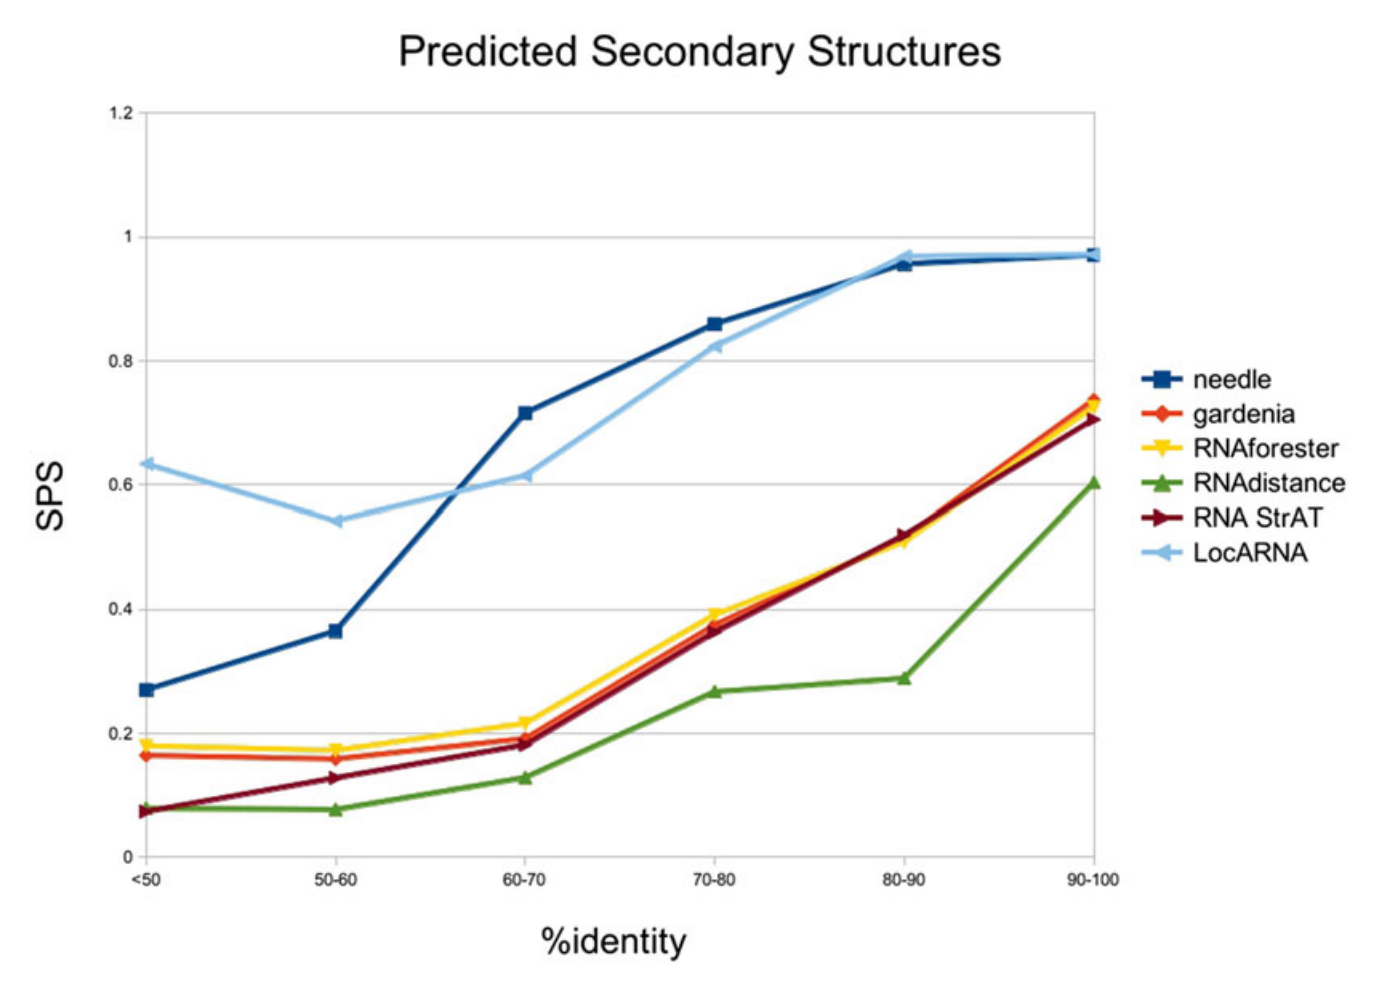
\includegraphics[width=\textwidth]{predicted}
\end{frame}


\begin{frame}[c]{}
    \center
    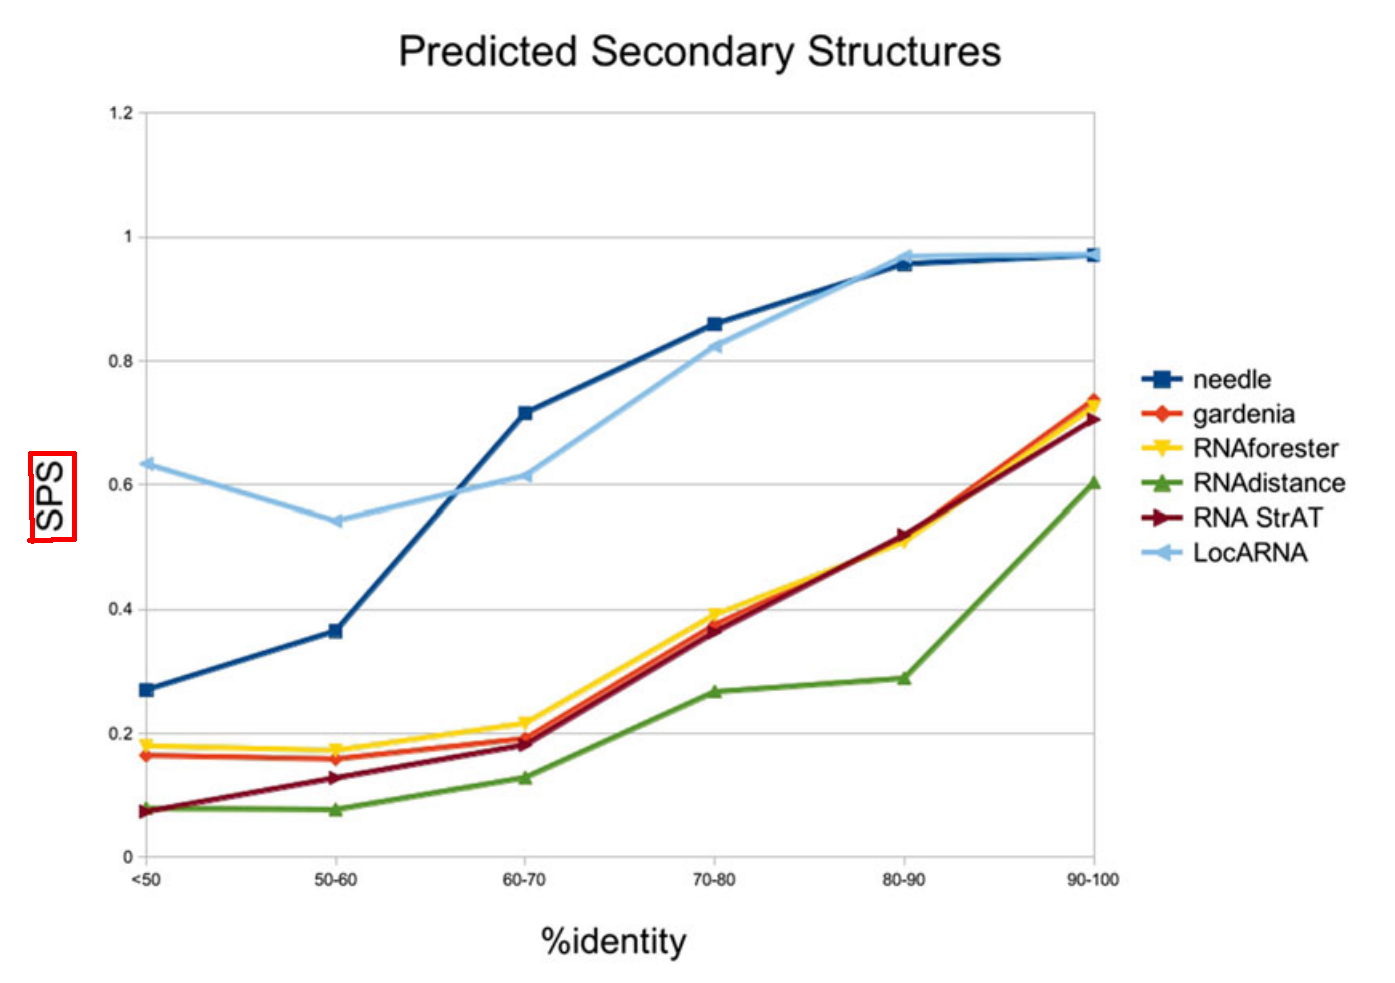
\includegraphics[width=\textwidth]{predicted_sps}
\end{frame}


\begin{frame}[c]{SPS - introduction}
    Sum of Pairs Score
    \newline
%    \vspace{2cm}
    \newline
    \pause
    Used to measure the \only<2-2>{alignment}\only<3->{similiarity} of two RNA sequences
\end{frame}


\begin{frame}[c]{Sequence Similiarity - Example}
    A: \only<4-5>{AAGGC}\only<1-1>{AAGGC}\only<2-3>{{\color{ForestGreen} AAGGC}}\only<1,4->{TT}\only<2-3>{{\color{red}TT}} \\
    B: \only<1-1>{AAGGC}\only<2-5>{{\color{ForestGreen} AAGGC}} \\
    C: \only<1-3>{AAGGC}\only<4->{{\color{ForestGreen} AAGGC}}\only<4-5>{{\color{red}AT}}\only<-3>{AT} \newline
    \newline
    Similiarity: \only<3,5>{60\% = 1 - (2 / 5) } \\
    1 - (edit distance / unaligned length of shorter sequence)
\end{frame}


\begin{frame}[c]{Sequence Similiarity - Example}
    A: {\color{ForestGreen}AAGGC}{\color{red}T}{\color{ForestGreen}T} \\
    B: AAGGC \\
    C: {\color{ForestGreen}AAGGC}{\color{red}A}{\color{ForestGreen}T} \newline
    \newline
    Similiarity: \only<2>{ 86\% = 1 - (1 / 7) } \\
    1 - (edit distance / unaligned length of shorter sequence)
\end{frame}


\begin{frame}[c]{}
    \center
    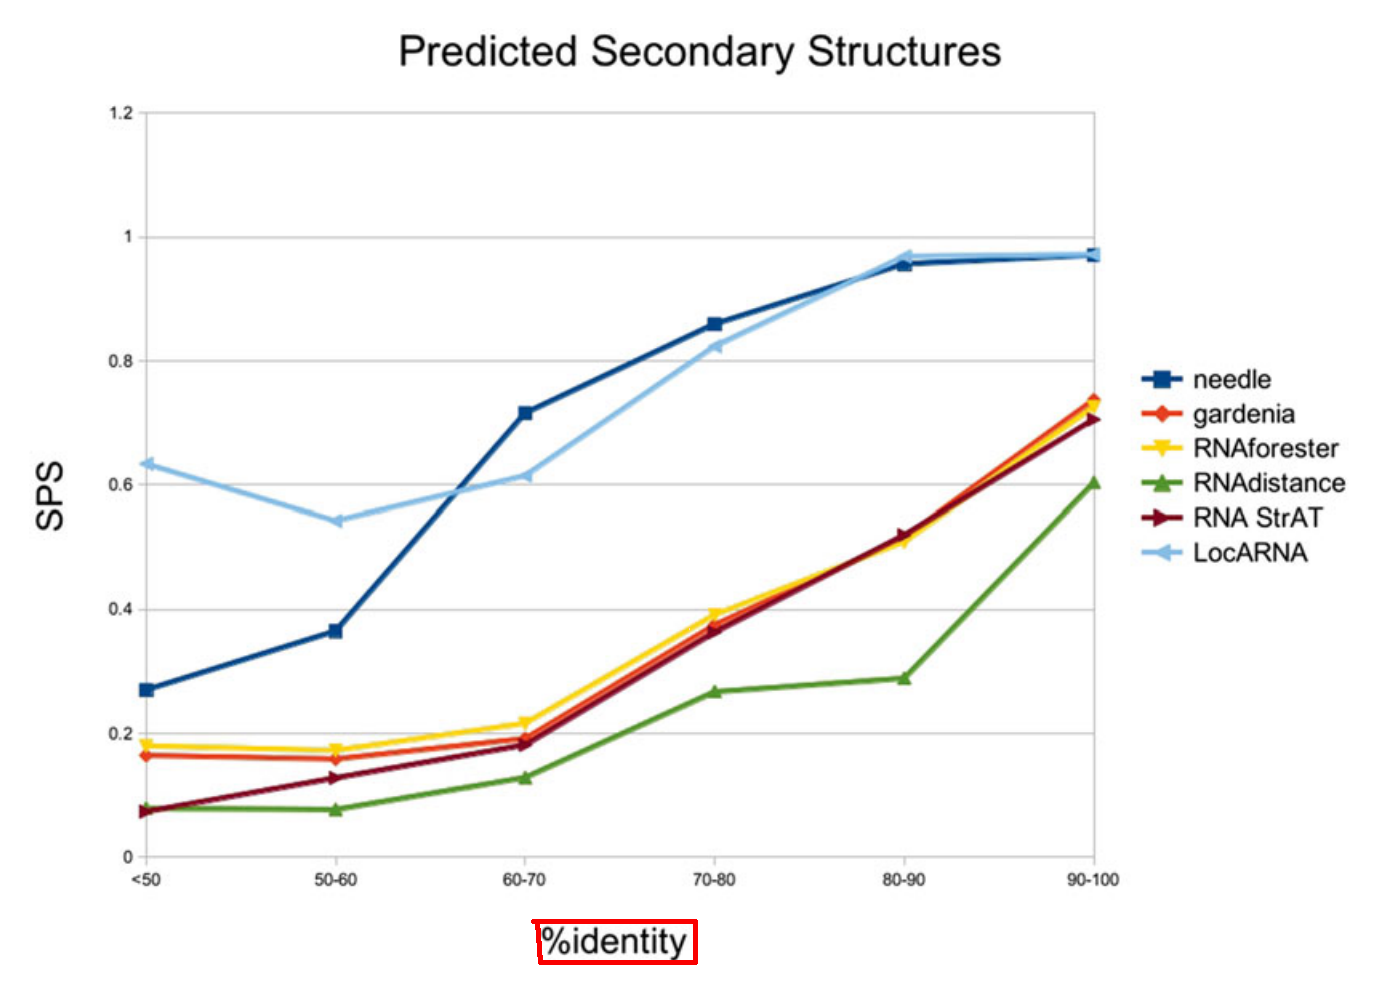
\includegraphics[width=\textwidth]{predicted_identity}
\end{frame}


\begin{frame}[c]{Sequence Identity - Example}
    A: \only<4-5>{AAGGC}\only<1-1>{AAGGC}\only<2-3>{{\color{ForestGreen} AAGGC}}TT \\
    B: \only<1-1>{AAGGC}\only<2-5>{{\color{ForestGreen} AAGGC}} \\
    C: \only<1-3>{AAGGC}\only<4-5>{{\color{ForestGreen} AAGGC}}AT \newline
    \newline
    Identity: \only<3,5>{100\%} \\
    Identical nucleotides / shorter sequence length
\end{frame}


\begin{frame}[c]{Sequence Identity - Example}
    A: {\color{ForestGreen}AAGGC}{\color{red}T}{\color{ForestGreen}T} \\
    B: AAGGC \\
    C: {\color{ForestGreen}AAGGC}{\color{red}A}{\color{ForestGreen}T} \newline
    \newline
    Identity: \only<2>{85\% = 6 / 7} \\
    Identical nucleotides / shorter sequence length
\end{frame}


\begin{frame}[c]{needle}
    \center
    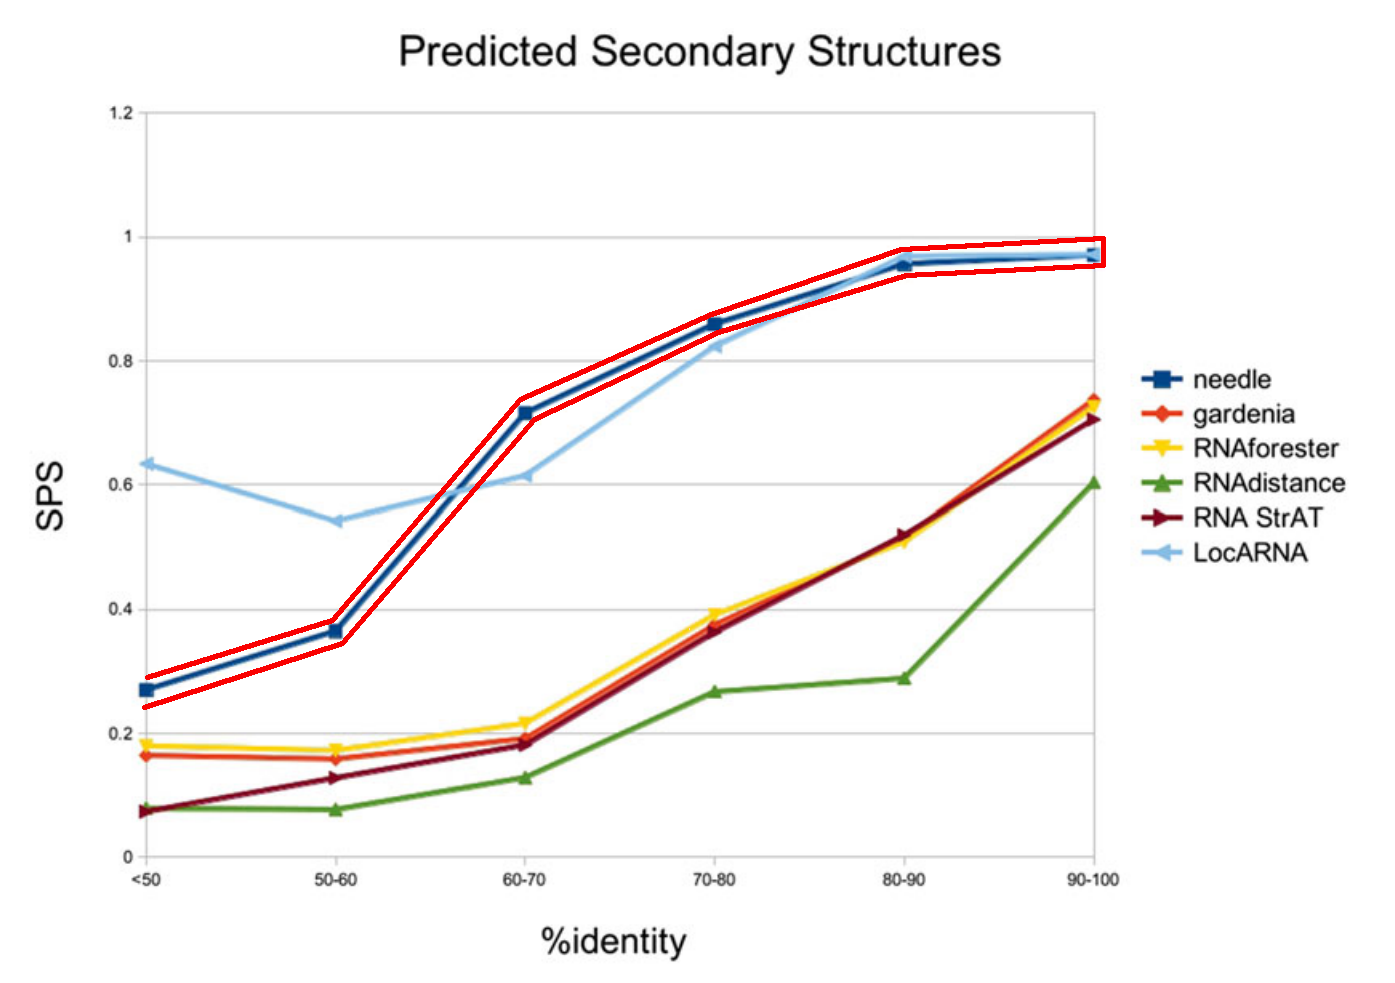
\includegraphics[width=\textwidth]{predicted_needle}
\end{frame}

\begin{frame}[c]{Needleman-Wunsch-Algorithm}
    \center
    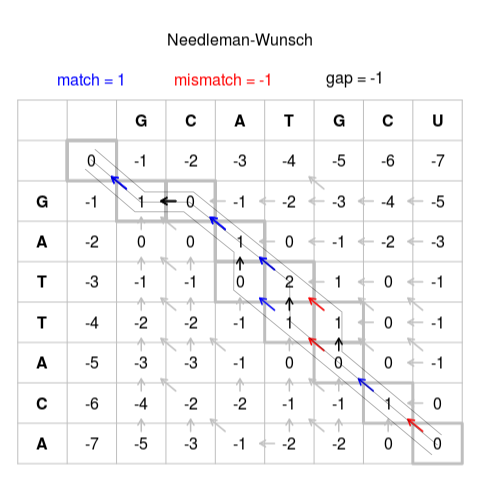
\includegraphics[width=0.75\textwidth]{Needleman-Wunsch_pairwise_sequence_alignment}
\end{frame}












\ifEnglish
%%%%%%%%%%%%%%%%%%%%%%%%%%%%%%%%%%%%%%%%%%%%%%%%%%%%%%%%%%%%

\section{Sources}

\begin{frame}[c]
    
\end{frame}



%%%%%%%%%%%%%%%%%%%%%%%%%%%%%%%%%%%%%%%%%%%%%%%%%%%%%%%%%%%%
\else
%%%%%%%%%%%%%%%%%%%%%%%%%%%%%%%%%%%%%%%%%%%%%%%%%%%%%%%%%%%%


%%%%%%%%%%%%%%%%%%%%%%%%%%CITES%%%%%%%%%%%%%%%%%%%%%%%%%%%%%
\section{Quellen}

%%%%%%%%%%%%%%%%%%%%%%%%%%CITES%%%%%%%%%%%%%%%%%%%%%%%%%%%%%
\begin{frame}[c,fragile,allowframebreaks]{Quellen}
    Die Folien sind zu finden unter: \newline
    \url{https://github.com/fkarg/things-to-talk-about/tree/master/lesswrong}
    \newline
    \newline
    Das Forum, mit diesen und sehr viel mehr Themen: \newline

% 
% 
%     Das Buch, aus dem ich den Vortrag gebastelt hab:
% 
    \beamertemplatearticlebibitems
    \begin{thebibliography}{10}
    \bibitem{Less Wrong}
            {\bf Less Wrong}
            \newblock \url{http://lesswrong.com/}

%     \beamertemplatebookbibitems
%     \bibitem{Richard Rumelt}
%         Richard Rumelt
%         \newblock {\em Good Strategy / Bad Strategy}.
%         \newblock The Difference and Why It Matters \\
%                   ISBN: 978-1-78125-154-6
%     \beamertemplatearticlebibitems
%     \bibitem{Lesswrong}
%         Lesswrong
%             \newblock {\em Expecting short Inferential Distances}
%             \newblock \url{http://lesswrong.com/lw/kg/expecting\_short\_inferential\_distances/}
%     \bibitem{Lesswrong}
%         Lesswrong
%             \newblock {\em Cached Thoughts}
%             \newblock \url{http://lesswrong.com/lw/k5/cached\_thoughts/}
%     \bibitem{Zenhabits}
%         Zenhabits
%             \newblock {\em say No so you can say YES}
%             \newblock \url{https://zenhabits.net/say-yes/}
% 
%     \bibitem{Wikiquote}
%         Fukuzawa Yukichi
%             \newblock {\em Wikiquote}
%             \newblock \url{https://en.wikiquote.org/wiki/Fukuzawa\_Yukichi}
% 
%     \bibitem{SpaceX}
%         SpaceX
%             \newblock {\em SpaceX}
%             \newblock \url{http://www.spacex.com/}
% 
%    \bibitem{Wihipedia}
%        Wikipedia
%            \newblock {\em Proton-M}
%            \newblock \url{https://en.wikipedia.org/wiki/Proton-M}
%    \bibitem{Wikipedia}
%        Wikipedia
%            \newblock {\em Ariane 5}
%            \newblock \url{https://en.wikipedia.org/wiki/Ariane\_5}
%    \bibitem{Wikipedia}
%        Wikipedia
%            \newblock {\em Delta IV Heavy}
%            \newblock \url{https://en.wikipedia.org/wiki/Delta\_IV}
   \end{thebibliography}
    % required the allowframebreaks for longer lists

\end{frame}



%%%%%%%%%%%%%%%%%%%%%%%%%%%%%%%%%%%%%%%%%%%%%%%%%%%%%%%%%%%%
\fi



% conter deklarieren
\newcounter{official}
\setcounter{official}{\value{page}}

%%%%%%%%%%%%%%%%%%%%%%%%%%%%%%%%%%%%%%%%%%%%%%%%%%%%%%%%%%%%%%%%%%%%%%%%%%%%%%%%%%%%%%%%%%%%%%%%%%%%%%%%%%%%%%%%%%%


\end{document}
